\chapter{Het p-blok I: de groepen van boor, koolstof en stikstof}\label{ch:b1:p-block-13-15}

De lucht die we inademen, bestaat voor vier vijfde uit stikstof, en toch
hebben planten er gebrek aan: de drievoudige binding \ce{N#N} is zo sterk
dat bijna niets haar verbreekt. Het grootste deel van de geschiedenis
kwam de stikstof van gewassen uit mest, uit bacteriën die op de wortels
van vlinderbloemigen leven, en uit gedolven nitraten. Begin twintigste
eeuw veranderde een reactie tussen stikstof en waterstof over een
ijzerkatalysator dat; vandaag maakt de wereld ongeveer 160 miljoen ton
stikstof per jaar als ammoniak, en ruwweg de helft van de stikstof in een
menselijk lichaam is ooit door een ammoniakfabriek gegaan. De \omterm{def:b1:periodicity:table}{groepen} 13,
14 en 15 bevatten de elementen van dat verhaal --- stikstof en fosfor voor
kunstmest, koolstof en silicium voor het leven en de gesteenten, boor en
aluminium voor glas en lichte legeringen. Dit hoofdstuk overloopt ze met
de werktuigen van de vorige hoofdstukken.

\begin{recall}
\omterm{def:b1:crystals-metals:allotropy}{Allotropen} van koolstof en de structuur van silicium en silica
(\cref{ch:b1:crystals-ionic-covalent}); het karakter van oxiden
(\cref{def:b1:s-block:oxide-character}); \omterm{def:b1:nernst:oxidation-number}{oxidatiegetallen} en
\omterm{def:b1:nernst:electrode-potential}{standaardpotentialen} (\cref{ch:b1:nernst}); \omterm{def:b1:precipitation:amphoteric-hydroxide}{amfotere hydroxiden}
(\cref{ch:b1:precipitation}); evenwichtsconstanten uit gibbsenergieën
(\cref{ch:b1:extent-q-and-k}).
\end{recall}
% ledger: usgs:N-world-2025

\begin{omfigure}
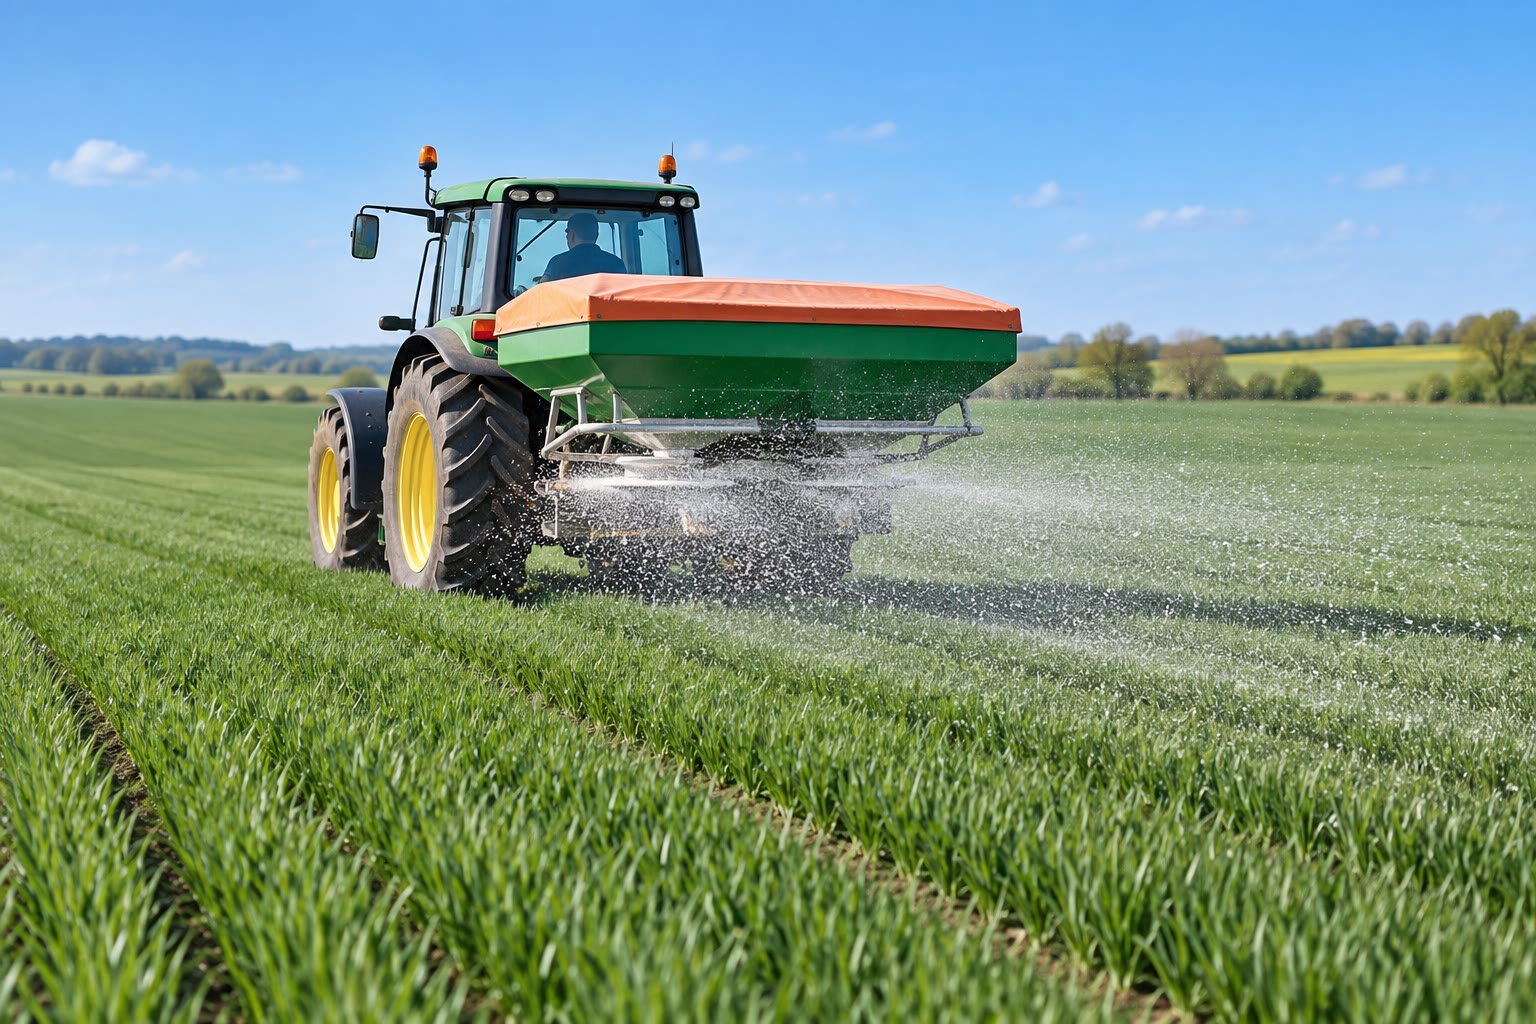
\includegraphics[width=0.55\linewidth]{images/book2/ai/b1-27-fertiliser-field.jpg}

{\small Een stikstofkunstmest wordt over een tarweveld uitgestrooid. Het
meeste ervan is via het haber-boschproces uit de stikstof van de lucht
gemaakt.}
\end{omfigure}

\section{Groep 13: boor en aluminium}

Boor is een \omterm{def:b1:periodicity:metalloid}{metalloïde} die covalente verbindingen met een onvolledig
octet vormt: in \ce{BF3} en boorzuur \ce{B(OH)3} heeft boor zes
\omterm{def:b1:quantum-numbers:configuration}{valentie-elektronen} en gedraagt het zich als een \omterm{def:b1:lewis-resonance-vsepr:lewis-acid}{lewiszuur}
(\cref{ch:b1:lewis-resonance-vsepr}). Boorzuur is een \omterm{def:b1:predominant-reaction:strong-acid}{zwak zuur}, niet
doordat het een proton afstaat, maar doordat het een hydroxide-ion
opneemt, \ce{B(OH)3 + 2H2O <=> B(OH)4- + H3O+}. Borax, een natriumboraat,
wordt gebruikt in glas en wasmiddelen.

\begin{definition}[Oxozuur]\label{def:b1:p-block-13-15:oxoacid}
Een \emph{oxozuur}\index{oxozuur} is een zuur waarin de zure
waterstofatomen gebonden zijn aan zuurstofatomen die aan een \omterm{def:b1:complexation:complex}{centraal
atoom} gebonden zijn: \ce{B(OH)3}, \ce{H2CO3}, \ce{HNO3} (\ce{HO-NO2}),
\ce{H3PO4} (\ce{(HO)3PO}), \ce{H2SO4}. Hoe meer zuurstofatomen zonder
waterstof rond het \omterm{def:b1:complexation:complex}{centrale atoom}, hoe sterker het zuur.
\end{definition}

Aluminium, onder boor, is een metaal, maar zijn kleine, sterk geladen ion
geeft het een \omterm{def:b1:s-block:oxide-character}{amfoteer oxide} en hydroxide (\cref{sec:b1:precipitation:amphoteric}).
Zijn erts is bauxiet, een mengsel van aluminiumhydroxiden met ijzeroxiden
en silica; in 2025 won de wereld ongeveer 440 miljoen ton bauxiet en
raffineerde ze er ongeveer 150 miljoen ton aluinaarde uit.
% ledger: usgs:bauxite-world-2025, usgs:alumina-world-2025

\begin{proposition}[Het bayerproces]\label{prop:b1:p-block-13-15:bayer}
Heet geconcentreerd natriumhydroxide lost het aluminium van bauxiet op
als \ce{Al(OH)4-} en laat de ijzeroxiden achter (rode modder); afkoelen en
enten van de gefiltreerde oplossing slaat zuiver \ce{Al(OH)3} neer, dat
tot aluinaarde gecalcineerd wordt, \ce{2Al(OH)3 -> Al2O3 + 3H2O}.
\end{proposition}

\begin{proof}
\ce{Al(OH)3(s) + OH- <=> Al(OH)4-} heeft $K = 10^{-1.23}$ bij
\qty{25}{\celsius} (\cref{ch:b1:precipitation}): bij een hoge \ce{[OH-]}
is het aluminium in oplossing, terwijl ijzer(III)hydroxide, dat niet
amfoteer is, vast blijft (\cref{exo:b1:precipitation:12}). Verdunnen en
afkoelen verlagen de \ce{[OH-]} en verschuiven het quotiënt zodat
$Q > K$ voor de omgekeerde reactie: het hydroxide slaat neer. Calcineren
verwijdert het water.
\end{proof}

Aluinaarde wordt daarna tot aluminium gereduceerd door elektrolyse in
gesmolten kryoliet, een industrie die in het deel van jaar~2 bestudeerd
wordt.

\begin{omfigure}
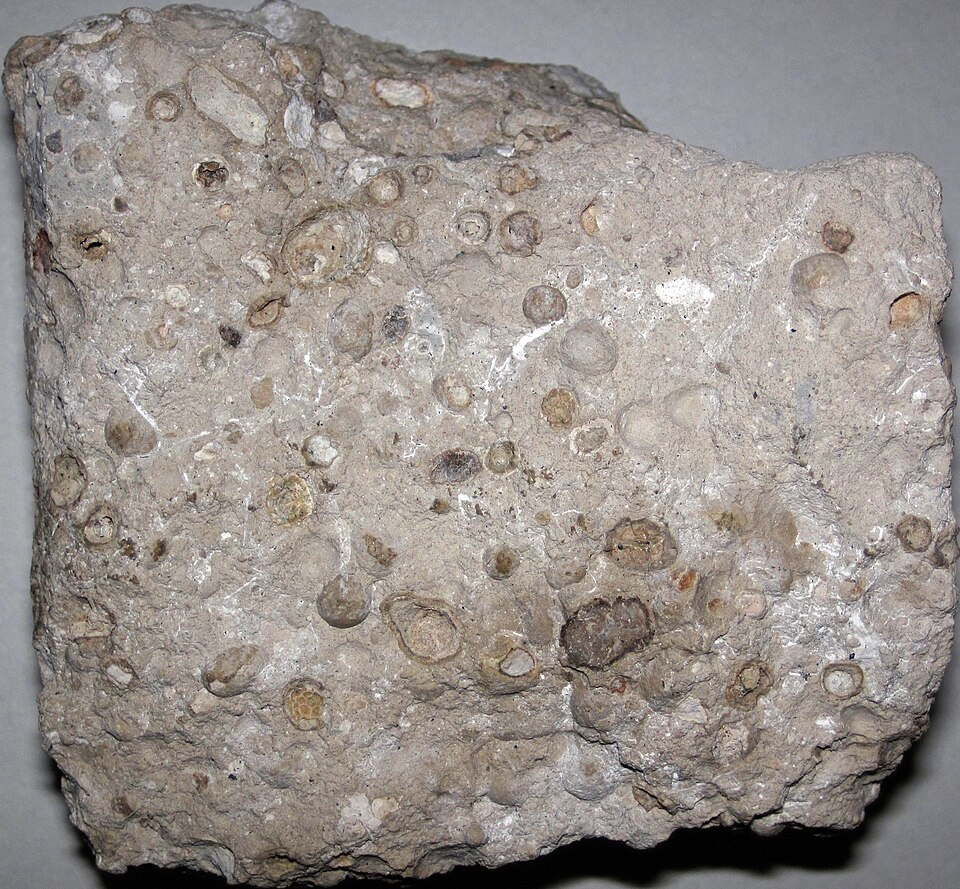
\includegraphics[height=3.6cm]{images/book2/bauxite.jpg}\hspace{0.4em}%
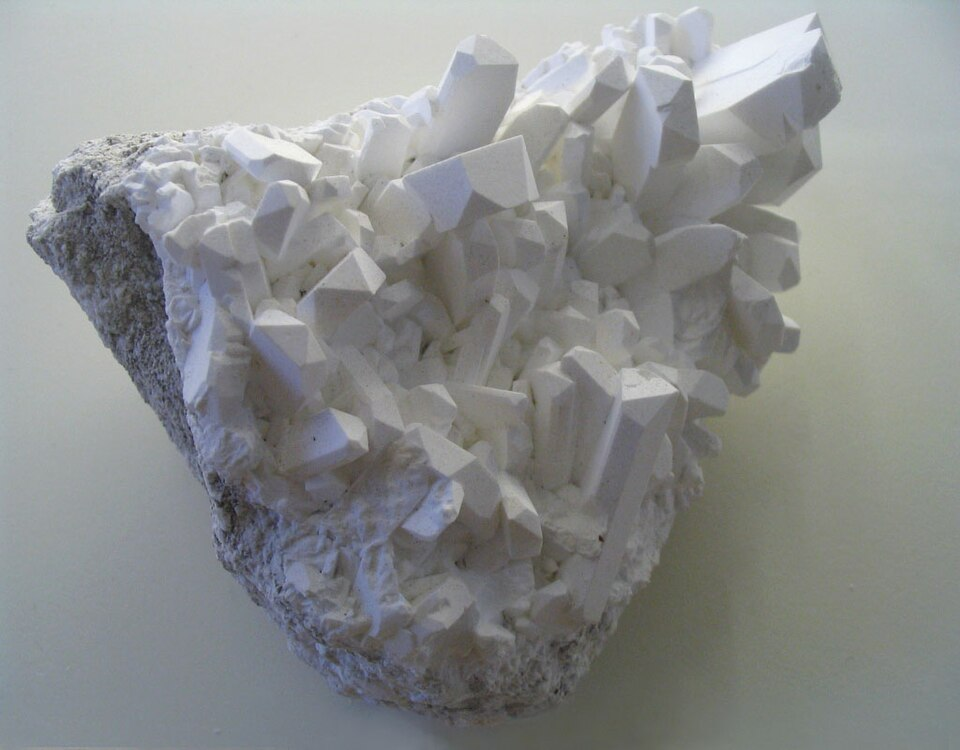
\includegraphics[height=3.6cm]{images/book2/borax.jpg}\hspace{0.4em}%
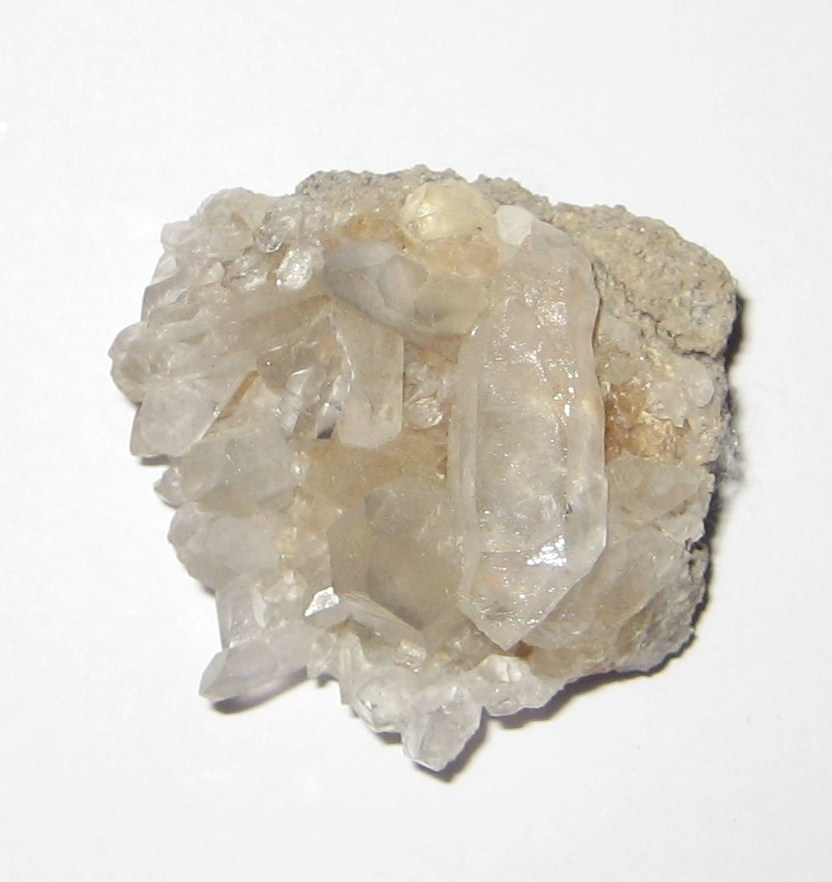
\includegraphics[height=3.6cm]{images/book2/quartz.jpg}\hspace{0.4em}%
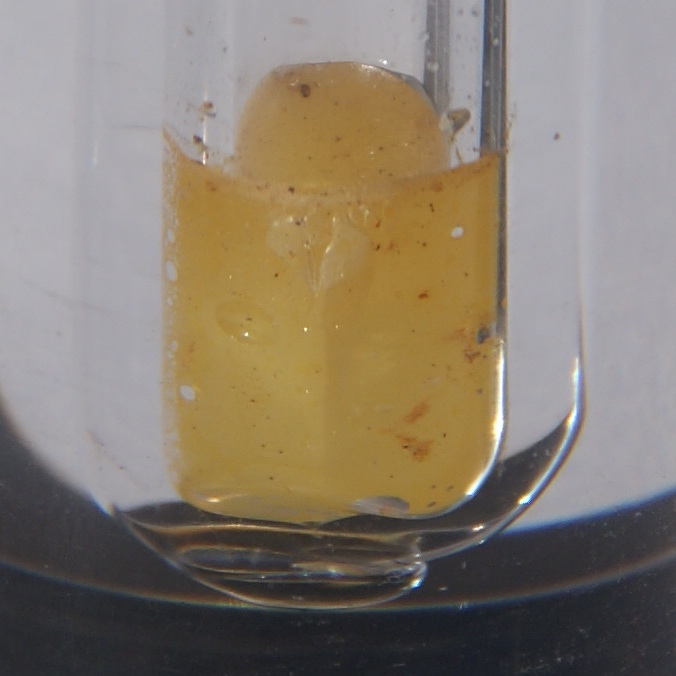
\includegraphics[height=3.6cm]{images/book2/white-phosphorus.jpg}

{\small Van links naar rechts: pisolitische bauxiet (James St. John, CC BY
2.0); boraxkristallen (Aram Dulyan, publiek domein); een groep
kwartskristallen, \ce{SiO2} (Stephanie Clifford, CC BY 2.0); witte fosfor,
met een beetje rode fosfor, onder water bewaard omdat hij aan de lucht
ontbrandt (Hi-Res Images of Chemical Elements, CC BY 3.0). Alle Wikimedia
Commons.}
\end{omfigure}

\section{Groep 14: koolstof en silicium}

Koolstof en silicium vormen allebei vier bindingen, maar op een andere
manier. Koolstof vormt sterke dubbele bindingen: \ce{CO2} is een molecuul,
\ce{O=C=O}, een gas. Silicium doet dat nauwelijks: \ce{SiO2} is een
covalent netwerk van \ce{SiO4}-tetraëders die al hun hoekpunten delen,
een harde vaste stof, kwarts (\cref{ch:b1:crystals-ionic-covalent}).
Koolstofdioxide is een \omterm{def:b1:s-block:oxide-character}{zuur oxide}, dat koolzuur, waterstofcarbonaten en
carbonaten geeft (\cref{ch:b1:predominant-reaction}); silica is ook een
\omterm{def:b1:s-block:oxide-character}{zuur oxide}, dat door gesmolten alkali aangetast wordt tot silicaten.

\begin{proposition}[Silicaateenheden]\label{prop:b1:p-block-13-15:silicate-units}
Silicaten zijn opgebouwd uit \ce{SiO4}-tetraëders; het aantal hoekpunten
dat met andere tetraëders gedeeld wordt, legt de formule van het anion
vast: geen, \ce{SiO4^4-} (geïsoleerde tetraëders); twee, ketens
$(\ce{SiO3})_n^{2n-}$; drie, lagen $(\ce{Si2O5})_n^{2n-}$; vier, het
neutrale raamwerk \ce{SiO2}.
\end{proposition}

\begin{proof}
Een gedeeld zuurstofatoom behoort voor de helft tot elke tetraëder. Een
tetraëder die $k$ hoekpunten deelt, bezit $4 - k$ zuurstofatomen volledig
en $k$ voor de helft: $4 -
k/2$ zuurstofatomen per siliciumatoom. Elk niet-gedeeld zuurstofatoom
draagt een lading $-1$ (het heeft één binding), elk gedeeld geen: de
lading per siliciumatoom is $-(4 - k)$. $k = 0$: \ce{SiO4^4-}; $k = 2$:
\ce{SiO3^2-} per siliciumatoom; $k = 3$: \ce{SiO_{2.5}^-}, dus
\ce{Si2O5^2-}; $k = 4$: \ce{SiO2}.
\end{proof}

\begin{omfigure}
\begin{tikzpicture}[font=\small, line join=round]
  % one SiO4 tetrahedron in perspective
  \begin{scope}
    \coordinate (t) at (0,1.2); \coordinate (a) at (-1.0,-0.5);
    \coordinate (b) at (1.0,-0.5); \coordinate (c) at (0.25,0.05);
    \draw[thick, omDef] (t) -- (a) -- (b) -- cycle; \draw[thick, omDef] (t) -- (b);
    \draw[dashed, omDef] (a) -- (c) -- (b) (t) -- (c);
    \foreach \p in {t,a,b,c} \shade[ball color=red!60] (\p) circle (0.16);
    \shade[ball color=gray!40] (0.06,0.18) circle (0.11);
    \node at (0,-1.2) {\ce{SiO4^4-}: één tetraëder};
  \end{scope}
  % a chain of tetrahedra seen from above
  \begin{scope}[xshift=3.6cm]
    \foreach \i in {0,1,2,3} {
      \draw[thick, omDef, fill=omDef!10] (\i*1.1,0) -- (\i*1.1+0.55,0.95) -- (\i*1.1+1.1,0) -- cycle;
      \shade[ball color=red!60] (\i*1.1+0.55,0.95) circle (0.12);
      \shade[ball color=red!60] (\i*1.1+0.55,0.32) circle (0.10);
    }
    \foreach \i in {0,1,2,3,4} \shade[ball color=red!60] (\i*1.1,0) circle (0.12);
    \node[align=center] at (2.2,-1.0) {keten $(\ce{SiO3})_n^{2n-}$: elke tetraëder\\ deelt twee hoekpunten (van bovenaf gezien)};
  \end{scope}
\end{tikzpicture}

{\small Silicaateenheden: een geïsoleerde \ce{SiO4}-tetraëder (silicium
grijs, zuurstof rood), en een keten waarin elke tetraëder twee
zuurstofatomen met zijn buren deelt. Lagen (drie gedeelde hoekpunten)
vormen mica's en kleien; een raamwerk (vier) vormt kwarts.}
\end{omfigure}

\begin{definition}[Effect van het inerte paar]\label{def:b1:p-block-13-15:inert-pair}
Het \emph{effect van het inerte paar}\index{effect van het inerte paar}
is de toenemende stabiliteit, naar beneden in de \omterm{def:b1:periodicity:table}{groepen} 13 tot 15, van
de oxidatietoestand die twee lager ligt dan de hoogste van de groep:
thallium(I) eerder dan (III), lood(II) eerder dan (IV), bismut(III)
eerder dan (V). Het \textit{ns}$^2$-paar van de zware elementen wordt
stevig vastgehouden en neemt weinig deel aan de binding.
\end{definition}

Het effect verklaart waarom lood(IV)oxide een sterke \omterm{def:b1:nernst:couple}{oxidator} is
($E^\circ(\ce{PbO2}/\ce{Pb^2+}) = 1.46$~V, \cref{ch:b1:nernst}), terwijl
koolstof(IV) en silicium(IV) de stabiele toestanden van hun elementen
zijn.

\section{Groep 15: stikstof}

\begin{proposition}[De stikstofladder]\label{prop:b1:p-block-13-15:nitrogen-ladder}
Stikstof neemt elk \omterm{def:b1:nernst:oxidation-number}{oxidatiegetal} van $-3$ tot $+5$ aan: \ce{NH3} en
\ce{NH4+} ($-$III), \ce{N2H4} ($-$II), \ce{NH2OH} ($-$I), \ce{N2} (0),
\ce{N2O} ($+$I), \ce{NO} ($+$II), \ce{HNO2} en \ce{NO2-} ($+$III),
\ce{NO2} ($+$IV), \ce{HNO3} en \ce{NO3-} ($+$V).
\end{proposition}

\begin{proof}
Pas de regels van \cref{prop:b1:nernst:on-rules} toe op elke formule, met
H op $+$I en O op $-$II: in \ce{N2H4}, $2x + 4 = 0$; in \ce{NO2-}, $x - 4 =
-1$; enzovoort.
\end{proof}

\begin{definition}[Stikstoffixatie]\label{def:b1:p-block-13-15:nitrogen-fixation}
\emph{Stikstoffixatie}\index{stikstoffixatie} is elk proces dat de
distikstof van de lucht omzet in een verbinding (ammoniak, nitraat) die
levende organismen of de industrie kunnen gebruiken: biologische
fixatie door bacteriën, fixatie door bliksem, en de industriële synthese
van ammoniak.
\end{definition}

Het haber-boschproces combineert stikstof en waterstof over een
ijzerkatalysator, \ce{N2 + 3H2 <=> 2NH3}. De reactie is bij
kamertemperatuur begunstigd ($K = 10^{5.8}$ bij \qty{25}{\celsius}, uit de
vormingsgibbsenergie van ammoniak), maar te traag; de \omterm{def:b1:elementary-steps:catalyst}{katalysator} werkt
alleen warm, en de keuze van temperatuur en druk die snelheid en
\omterm{def:b1:extent-q-and-k:fractional-extent}{rendement} verzoent, wordt in het deel van jaar~2 gemaakt. Ammoniak wordt
daarna via het ostwaldproces tot salpeterzuur geoxideerd.
% ledger: dfg:NH3_g

\begin{omfigure}
\begin{tikzpicture}[font=\small, >={Stealth}, box/.style={draw, rounded corners, fill=omDef!8, align=center, minimum height=0.9cm}]
  \node[box] (air) at (0,0) {lucht\\\ce{N2}};
  \node[box] (gas) at (0,-1.6) {aardgas\\\ce{H2}};
  \node[box] (hb) at (3.4,-0.8) {Haber--Bosch\\ijzerkatalysator};
  \node[box] (ox1) at (7.3,-0.8) {Pt--Rh-gaas\\\ce{NH3} $\to$ \ce{NO}};
  \node[box] (ox2) at (11.0,-0.8) {oxidatie\\absorptie\\\ce{NO} $\to$ \ce{NO2} $\to$ \ce{HNO3}};
  \draw[->, thick] (air) -- (hb);
  \draw[->, thick] (gas) -- (hb);
  \draw[->, thick] (hb) -- node[above] {\ce{NH3}} (ox1);
  \draw[->, thick] (ox1) -- node[above] {\ce{NO}} (ox2);
  \draw[->, thick] (ox2.south) -- ++(0,-0.6) node[below] {\ce{HNO3}};
  \draw[->, thick] (hb.south) -- ++(0,-0.9) node[below] {\ce{NH3} (kunstmest)};
  \draw[->, thick] (ox2.north) -- ++(0,0.5) -| node[pos=0.25, above] {\ce{NO} gerecycleerd} (ox1.north);
\end{tikzpicture}

{\small Van lucht naar salpeterzuur: de ammoniaksynthese gevolgd door de
drie stappen van het ostwaldproces.}
\end{omfigure}

\begin{method}[Gekoppelde industriële vergelijkingen kloppend maken]\label{met:b1:p-block-13-15:ostwald-balance}
\begin{enumerate}
  \item Maak elke stap kloppend: (1) \ce{4NH3 + 5O2 -> 4NO + 6H2O};
        (2) \ce{2NO + O2 -> 2NO2}; (3) \ce{3NO2 + H2O -> 2HNO3 + NO}.
  \item Vermenigvuldig de stappen zodat elk gevormd intermediair verbruikt
        wordt (de \ce{NO} van stap 3 keert terug naar stap 2).
  \item Tel op: bij volledige recyclage van NO is de totale vergelijking
        \ce{NH3 + 2O2 -> HNO3 + H2O}, één salpeterzuur per ammoniak.
  \item Gebruik de totale vergelijking voor massabalansen, de stappen voor
        het ontwerp van elke reactor.
\end{enumerate}
\end{method}

\begin{history}[Fritz Haber]
\begin{minipage}[t]{0.18\linewidth}\vspace{0pt}
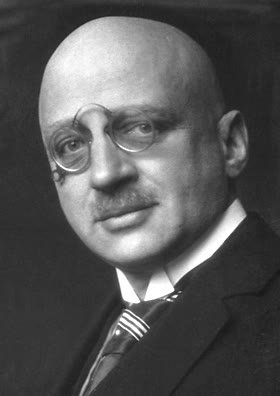
\includegraphics[width=\linewidth]{images/book2/haber.jpg}
\end{minipage}\hfill
\begin{minipage}[t]{0.78\linewidth}\vspace{0pt}
Fritz Haber toonde aan dat ammoniak onder druk over een \omterm{def:b1:elementary-steps:catalyst}{katalysator} uit
stikstof en waterstof gemaakt kon worden; Carl Bosch maakte van de
laboratoriumreactie een industrieel proces. Haber kreeg de Nobelprijs
voor Scheikunde van 1918. Dezelfde man leidde in de Eerste Wereldoorlog
de eerste grootschalige inzet van chloor als wapen: de chemie die de
helft van de mensheid voedt en de chemie die doodt, worden gescheiden
door de keuzes van chemici. (Foto: The Nobel Foundation, gepubliceerd in
1919, publiek domein, Wikimedia Commons.)
\end{minipage}
\end{history}

\section{Fosfor en de trends naar beneden in de groepen}

Fosfor, onder stikstof, vormt geen drievoudige bindingen \ce{P#P}: witte
fosfor bestaat uit \ce{P4}-tetraëders, gespannen en reactief (hij
ontbrandt aan de lucht en wordt onder water bewaard); rode fosfor is een
polymeer, veel minder reactief. Verbranden van fosfor geeft \ce{P4O10},
het zuurste van de gewone oxiden, dat met water fosforzuur geeft,
$\mathrm{p}K_a$ 2.15, 7.21, 12.34 (\cref{ch:b1:predominant-reaction}).
Fosfaaterts, waarvan in 2025 ongeveer 250 miljoen ton gewonnen werd, wordt
met zwavelzuur omgezet in fosfaatkunstmest.
% ledger: usgs:phosphate-world-2025

Naar beneden in elke groep worden de elementen metallischer (van boor
naar thallium, van koolstof naar lood, van stikstof naar bismut), hun
oxiden basischer, en de lagere oxidatietoestanden stabieler: het \omterm{def:b1:p-block-13-15:inert-pair}{effect
van het inerte paar}. Door een \omterm{def:b1:periodicity:table}{periode} heen worden de oxiden zuurder, van
het basische \ce{Na2O} tot de \omterm{def:b1:s-block:oxide-character}{zure oxiden} van fosfor en zwavel.

\section{Oefeningen}

\begin{exercise}[$\star$]\label{exo:b1:p-block-13-15:1}
Geef het \omterm{def:b1:nernst:oxidation-number}{oxidatiegetal} van stikstof in \ce{NH4NO3} (beide atomen),
\ce{N2O5}, \ce{HNO2}, \ce{N2H4} en \ce{Mg3N2}.
\end{exercise}

\begin{exercise}[$\star$]\label{exo:b1:p-block-13-15:2}
Teken de lewisstructuren van \ce{BF3}, \ce{NH3} en van het adduct
\ce{F3B-NH3}; duid het \omterm{def:b1:lewis-resonance-vsepr:lewis-acid}{lewiszuur} en de \omterm{def:b1:lewis-resonance-vsepr:lewis-acid}{lewisbase} aan.
\end{exercise}

\begin{exercise}[$\star$]\label{exo:b1:p-block-13-15:3}
Schrijf de reacties op van \ce{CO2}, \ce{SiO2} (gesmolten) en \ce{P4O10}
met natriumhydroxide, en van \ce{Al2O3} met een zuur en met een base.
\end{exercise}

\begin{exercise}[$\star$]\label{exo:b1:p-block-13-15:4}
Bereken de evenwichtsconstante van \ce{N2 + 3H2 <=> 2NH3} bij
\qty{25}{\celsius} uit $\Delta_f G^\circ(\ce{NH3}) =
\qty{-16.45}{kJ/mol}$.
\end{exercise}

\begin{exercise}[$\star\star$]\label{exo:b1:p-block-13-15:5}
Geef met de telling van \cref{prop:b1:p-block-13-15:silicate-units} de
formule van een ring van zes tetraëders die elk twee hoekpunten delen
(zoals in beryl) en van een dubbele keten waarin de helft van de
tetraëders twee hoekpunten deelt en de andere helft drie.
\end{exercise}

\begin{exercise}[$\star\star$]\label{exo:b1:p-block-13-15:6}
Bereken de massa aluinaarde die verkregen wordt uit één ton bauxiet met
\qty{55}{\percent} \ce{Al(OH)3} in massa, bij een terugwinning van
\qty{92}{\percent}.
\end{exercise}

\begin{exercise}[$\star\star$]\label{exo:b1:p-block-13-15:7}
Toon aan dat boorzuur eerder een \omterm{def:b1:lewis-resonance-vsepr:lewis-acid}{lewiszuur} dan een \omterm{def:b1:predominant-reaction:bronsted}{brønstedzuur} is, en
verklaar waarom zijn oplossing toch zuur is.
\end{exercise}

\begin{exercise}[$\star\star$]\label{exo:b1:p-block-13-15:8}
Maak de oxidatie van ammoniak tot \ce{NO} kloppend met de
\omterm{def:b1:nernst:oxidation-number}{oxidatiegetallen} en geef het aantal uitgewisselde elektronen per
\ce{NH3}.
\end{exercise}

\begin{exercise}[$\star\star$]\label{exo:b1:p-block-13-15:9}
Ammoniumnitraat wordt gemaakt uit ammoniak en salpeterzuur. Schrijf de
reactie op, en bereken de massa ammoniak die per ton ammoniumnitraat
nodig is (zowel voor het salpeterzuur als voor de neutralisatie).
\end{exercise}

\begin{exercise}[$\star\star\star$]\label{exo:b1:p-block-13-15:10}
Verklaar met de sterkte van $\pi$-bindingen tussen atomen van de tweede
en van de derde \omterm{def:b1:periodicity:table}{periode} waarom stikstof een tweeatomig gas is en fosfor
een vaste stof uit \ce{P4}-moleculen, en waarom koolstofdioxide een gas
is en silica een vaste stof.
\end{exercise}

\begin{exercise}[$\star\star\star$]\label{exo:b1:p-block-13-15:11}
Toon met de \omterm{def:b1:nernst:electrode-potential}{standaardpotentialen} aan dat lood(IV)oxide in zuur milieu
chloride-ionen tot chloor oxideert, terwijl silicium(IV)oxide niets van
dien aard doet. Leg het verband met het \omterm{def:b1:p-block-13-15:inert-pair}{effect van het inerte paar}.
\end{exercise}

\begin{exercise}[$\star\star\star$]\label{exo:b1:p-block-13-15:12}
De wereld produceerde in 2025 ongeveer 160 miljoen ton stikstof als
ammoniak. Welke massa ammoniak is dat, en welke massa waterstof bevatte
die? Waar komt die waterstof vooral vandaan?
\end{exercise}

\section{Probleem: van lucht tot kunstmest}

\begin{problem}[{Weekendprobleem --- de drievoudige binding van stikstof,
de ammoniaksynthese, de drie stappen van de productie van salpeterzuur,
ammoniumnitraat, en de massa salpeterzuur die uit één ton ammoniak
verkregen kan worden}]
\label{pb:b1:p-block-13-15:1}
Een kunstmestfabriek zet ammoniak om in salpeterzuur en ammoniumnitraat.
Molaire massa's (\unit{g/mol}): \ce{N2} 28.0, \ce{H2} 2.0, \ce{NH3}
17.0, \ce{HNO3} 63.0, \ce{NH4NO3} 80.0, \ce{O2} 32.0;
$\Delta_f G^\circ(\ce{NH3(g)}) = \qty{-16.45}{kJ/mol}$ bij
\qty{25}{\celsius}.

\medskip
\noindent\textbf{Deel I --- Stikstof.}
\begin{enumerate}
  \item Teken de \omterm{def:b1:lewis-resonance-vsepr:lewis}{lewisstructuur} van \ce{N2} en zeg waarom het weinig
        reactief is.
  \item Geef het \omterm{def:b1:nernst:oxidation-number}{oxidatiegetal} van N in \ce{N2}, \ce{NH3}, \ce{NO},
        \ce{NO2}, \ce{HNO3} en \ce{NH4NO3}.
  \item Noem drie natuurlijke of industriële manieren om stikstof te
        fixeren.
  \item Waarom kunnen planten \ce{N2} niet rechtstreeks gebruiken?
  \item Welk element wordt geoxideerd en welk gereduceerd bij de synthese
        van ammoniak?
  \item Schrijf de synthese van ammoniak op.
\end{enumerate}

\medskip
\noindent\textbf{Deel II --- Ammoniak.}
\begin{enumerate}[resume]
  \item Bereken de evenwichtsconstante van de synthese bij
        \qty{25}{\celsius}.
  \item Waarom wordt de synthese toch warm uitgevoerd, over een
        \omterm{def:b1:elementary-steps:catalyst}{katalysator}?
  \item Bereken de massa's \ce{N2} en \ce{H2} voor één ton ammoniak.
  \item Welk volume lucht (\qty{78}{\percent} \ce{N2} in volume, ideaal
        gas, \qty{25}{\celsius}, \qty{1}{bar}) bevat die stikstof?
  \item Waar komt de waterstof vandaan?
  \item Waarom wordt ammoniak zelf in sommige landen als kunstmest
        gebruikt, en waarom wordt het vaak eerst omgezet?
\end{enumerate}

\medskip
\noindent\textbf{Deel III --- Salpeterzuur.}
\begin{enumerate}[resume]
  \item Maak stap 1, \ce{NH3 + O2 -> NO + H2O}, kloppend met \omterm{def:b1:nernst:oxidation-number}{oxidatiegetallen}. % ce-unbalanced-ok
  \item Maak stap 2, \ce{NO + O2 -> NO2}, kloppend. % ce-unbalanced-ok
  \item Maak stap 3, \ce{NO2 + H2O -> HNO3 + NO}, kloppend. Welk soort % ce-unbalanced-ok
        redoxreactie is het?
  \item Combineer de stappen, met volledige recyclage van NO, tot de
        totale vergelijking.
  \item Bereken de massa zuurstof die per ton ammoniak verbruikt wordt.
  \item Waarom gebruikt men in stap 1 een gaas van platina--rodium?
\end{enumerate}

\medskip
\noindent\textbf{Deel IV --- Ammoniumnitraat en massabalansen.}
\begin{enumerate}[resume]
  \item Schrijf de vorming van ammoniumnitraat op.
  \item Welke fractie van de ammoniak moet in salpeterzuur omgezet worden
        om alleen ammoniumnitraat te maken?
  \item Bereken de massa ammoniumnitraat uit één ton ammoniak die op die
        manier verdeeld wordt.
  \item Welk massapercentage stikstof bevat ammoniumnitraat?
  \item Waarom moet ammoniumnitraat ver van brandstoffen en warmte
        opgeslagen worden?
  \item Bereken de massa salpeterzuur die uit één ton ammoniak verkregen
        kan worden (volledige omzetting).
\end{enumerate}
\end{problem}
